% Topic control -- main section for Report 2 (final corrected version, 2026-10-29).
% Every number is from results/topic_control_revision/ (see report_revision_guide.md).
% Needs: booktabs, float ([H]), graphicx, amsmath. Figures are referenced as figures/<name>.png;
% copy them from results/topic_control_revision/figures/.
% Supplementary tables/figures (Tables tc-thresholds, tc-within; Figures tc-gee, tc-length)
% are in topic_control_appendix.tex, which must be \input in the same document.

\subsection*{Topic Control and Follow-up in Mixed-Gender Dyads}

Topic control is an important aspect of who dominates a conversation. The speaker whose topics the other person picks up usually steers the direction of the conversation. A long-standing idea in language and gender research is that men's topics are more likely to be taken up, whereas women's topics are more likely to be ignored or dropped.

Recent studies suggest that gender still shapes topic initiation \cite{TopicInitiationbyKoreanandChineseSpeakersonRealityDatingShows}, but large-scale studies indicate that gendered speech patterns depend on context and are not always male-dominated \cite{yoo2022conversational}. We test whether this pattern also appears in Indian podcasts (English and Hindi) featuring one host and one guest. Podcasts are well suited to this question because they include long and natural conversations between speakers. In addition, hosts also steer the discussion by asking questions and guests answer them. This helps us examine whether follow-up is associated with the speaker's gender or with their conversational role.

Our analysis focuses on mixed-gender host-guest conversations and compares how often male-initiated topics receive follow-up with how often female-initiated topics do. Since podcast transcripts do not label where the topic changes, topic initiation and follow-up are identified automatically using lexical similarity between conversational turns, with semantic similarity used as a robustness check.

\begin{quote}
\textbf{RQ:} In mixed-gender host--guest conversations, are topics introduced by male speakers followed up more often than topics introduced by female speakers?
\vspace{-0.8em}
\end{quote}

Based on prior research, we develop the following hypotheses:
\vspace{-0.8em}
\begin{quote}
\textbf{H$_1$:} Male-initiated topics are followed up more than female-initiated topics.

\textbf{H$_0$:} Male-initiated topics are not followed up more than female-initiated topics.
\end{quote}

The hypothesis test uses the \textbf{131 mixed-gender episodes} (67 MF + 64 FM; 262 speakers), which contain \textbf{17,046 topic initiations} with a response: \textbf{8,742 by male speakers} and \textbf{8,304 by female speakers}. Each of these episodes has one male and one female speaker, and also one host and one guest. This means that within an episode, gender and role are perfectly linked. So the only way to compare men and women in the same role is to compare different episodes (male-hosted vs.\ female-hosted).

\subsubsection*{Identifying initiations and follow-ups}
Consecutive lines from the same speaker are merged into one turn, and backchannels such as ``yeah'' and ``mhm'' are removed. Each turn is then represented as a TF-IDF vector, and the similarity between turns is measured with cosine similarity. A turn is treated as starting a new topic when its similarity to the previous turn is at or below the episode median. It is considered followed up when the other speaker's next turn is more similar to it than the median. Using a separate median for each episode makes the measure easier to compare across episodes.

However, most consecutive turns share no content words, so the median is often zero. In 72 of the 131 episodes, ``followed up'' simply means that the reply shares at least one content word with the turn before it. Therefore, this \textbf{automated lexical follow-up} measure captures lexical uptake between adjacent turns rather than topic change as a listener would judge it. It has not been checked against human judgements.

\subsubsection*{Statistical Analysis}
Since turns from the same episode are not independent, our main test is a \textbf{GEE logistic regression} that predicts follow-up from the initiator's gender, controls for role (host or guest) and turn length, and groups errors by episode. Since gender and role are linked within an episode, the gender result from this model depends on comparing male-hosted and female-hosted episodes. Therefore, we also ran a \textbf{sensitivity analysis}, where we changed one choice at a time: how turn length is included, how episodes are weighted, and whether errors are grouped by host instead of episode. We also directly compared the host--guest gap in male-hosted and female-hosted episodes.

We also report paired tests comparing the male and female speakers in the same episode, and a mixed-effects model. These answer slightly different questions: the paired tests do not control for role, and the mixed model uses the continuous similarity score instead of the yes/no follow-up. Additionally, we repeat the paired test using sentence embeddings, which capture meaning rather than word overlap.

\subsubsection*{Findings}

\paragraph{Raw comparison:}
After pooling across all initiations, male-initiated topics appear to be followed up more often (42.2\% vs.\ 37.7\%, a gap of \textbf{+4.4 pp}; Table~\ref{tab:tc-descriptive}). This pooled gap appears at every fixed similarity threshold (Appendix Table~\ref{tab:tc-thresholds}), but it does not take role into account. Within the same episode, there is no clear gap (41.5\% vs.\ 42.6\%). Fig.~\ref{fig:tc-episode} shows why: the male speaker is followed up more when he is the host (+9.4 pp) and less when he is the guest ($-12.3$ pp), and these cancel out.

\begin{table}[H]
\centering
\caption{Automated lexical follow-up rate by initiator gender in the 131 mixed-gender episodes (17,046 initiations). \emph{Pooled}: share of all initiations followed up; 95\% CIs from 5,000 bootstrap resamples of episodes. \emph{Per episode}: mean and median of each speaker's episode-level rate; $t$-based 95\% CIs. Not adjusted for role.}
\label{tab:tc-descriptive}
\begin{tabular}{lcccc}
\toprule
 & \multicolumn{2}{c}{Pooled} & \multicolumn{2}{c}{Per episode} \\
\cmidrule(lr){2-3}\cmidrule(lr){4-5}
Initiator & Initiations & Follow-up rate & Mean & Median \\
\midrule
Female & 8,304 & 37.7\% [35.7, 40.0] & 42.6\% [40.6, 44.7] & 43.3\% \\
Male   & 8,742 & 42.2\% [40.5, 43.9] & 41.5\% [39.8, 43.2] & 40.6\% \\
\midrule
Male $-$ female & & $+4.4$ pp [$+1.9$, $+6.7$] & \multicolumn{2}{c}{$-1.2$ pp [$-4.1$, $+1.8$]} \\
\bottomrule
\end{tabular}
\end{table}

\begin{figure}[H]
\centering
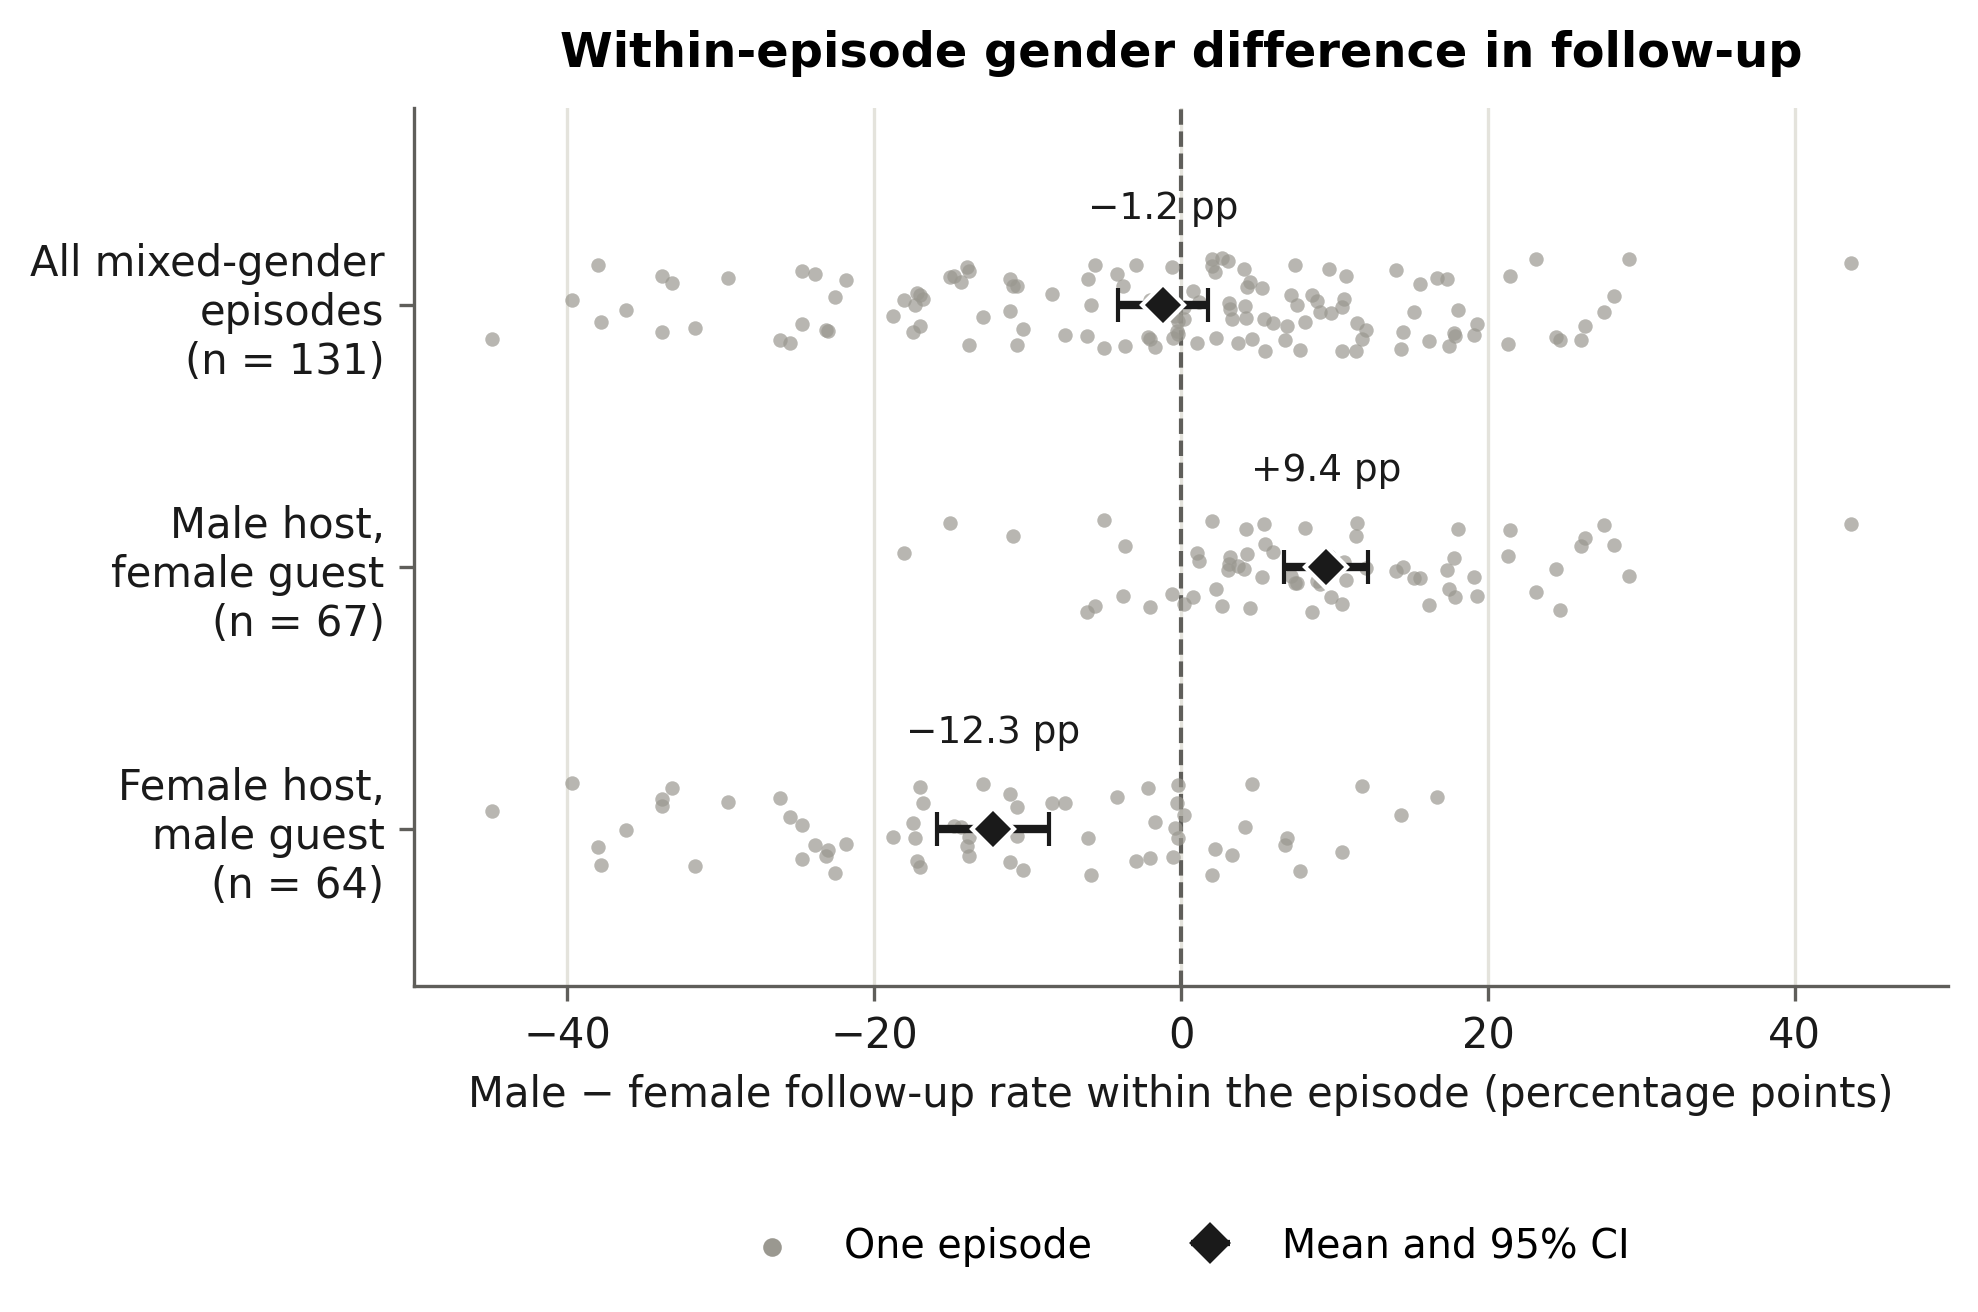
\includegraphics[width=0.65\linewidth]{figures/fig3_within_episode_gender_difference.png}
\caption{Within-episode male $-$ female difference in automated lexical follow-up rate (percentage points), for all 131 mixed-gender episodes and split by host gender (67 male-hosted, 64 female-hosted). Points are episodes; diamonds and bars are means with $t$-based 95\% CIs. Not adjusted for role: the male speaker is the host in male-hosted episodes and the guest in female-hosted ones.}
\label{fig:tc-episode}
\end{figure}

\paragraph{Role composition and the pooled gap:}
78\% of male initiations come from hosts, whereas only 30\% of female initiations do. So the pooled gender difference is strongly confounded by who is the host: it mostly compares hosts with guests. Within each role, the difference between men and women is small (hosts: 49\% female vs.\ 46\% male; guests: 36\% vs.\ 37\%; Fig.~\ref{fig:tc-role}). However, these men and women come from different episodes and shows, not the same conversation, so this comparison does not separate gender from show.

\begin{figure}[H]
\centering
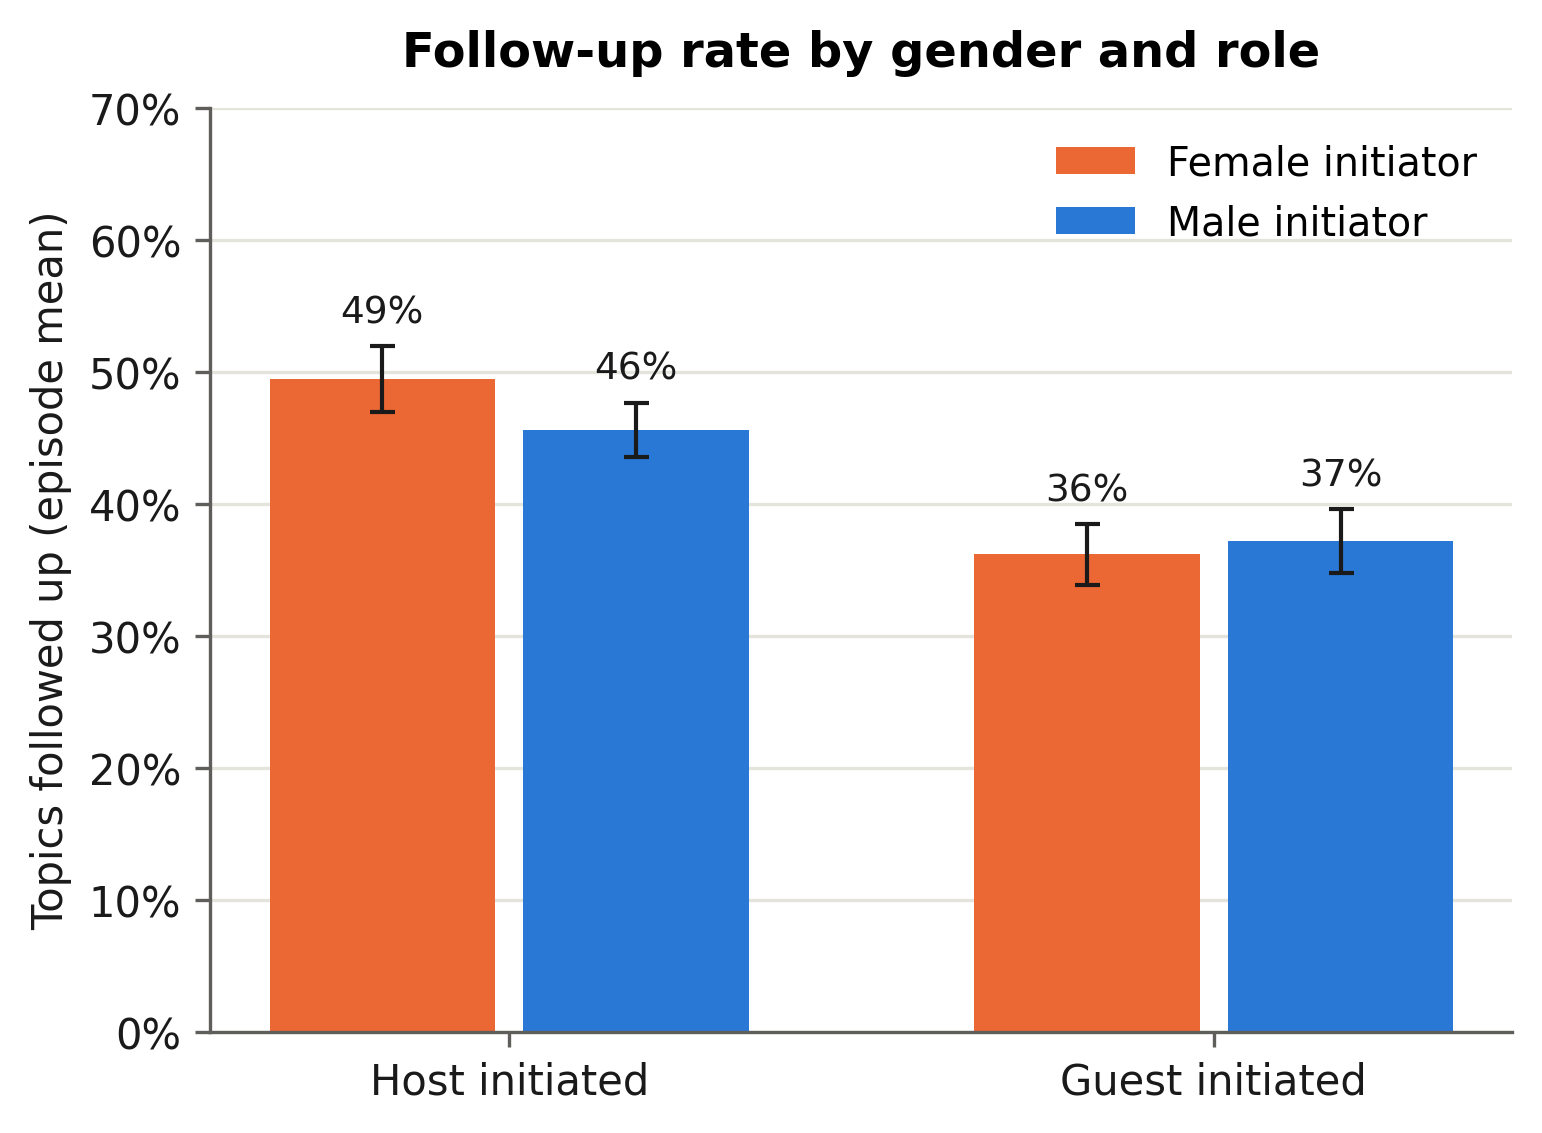
\includegraphics[width=0.6\linewidth]{figures/fig2_followup_by_gender_within_role.png}
\caption{Automated lexical follow-up rate by initiator gender within each role (131 mixed-gender episodes). Female hosts and male guests come from the 64 female-hosted episodes; male hosts and female guests from the 67 male-hosted episodes, so each gender comparison is between different episodes. Bars are means of episode-level rates with $t$-based 95\% CIs. Unadjusted.}
\label{fig:tc-role}
\end{figure}

\paragraph{Hypothesis test:}
The results do not support H$_1$ (Table~\ref{tab:tc-models}; Appendix Fig.~\ref{fig:tc-gee}). Host-initiated topics have higher odds of lexical follow-up than guest-initiated topics (OR $= 2.20$). In the original model, male-initiated topics have slightly lower odds of follow-up (OR $= 0.85$, $p = 0.002$), which is the opposite of what H$_1$ predicts.

However, the sensitivity analysis shows that this gender result is not robust (Table~\ref{tab:tc-sensitivity}, Fig.~\ref{fig:tc-sensitivity}). The odds ratio for men ranges from \textbf{0.79 to 1.00} depending on how turn length is included, and it is not significant when turn length is left out ($p = 0.94$), when reply length is added ($p = 0.13$), or when errors are grouped by host ($p = 0.08$). The direct episode-level comparison also finds no clear difference ($p = 0.22$). In contrast, the host association stays above 1 in every version (OR 1.50--2.78). The paired tests and the mixed model also find no clear gender difference ($p = 0.44$ and $p = 0.42$; Appendix Table~\ref{tab:tc-within}), although they answer slightly different questions. \textbf{We therefore do not reject H$_0$}, and we do not treat the OR of 0.85 as evidence that men's topics are followed up less. A non-significant result here also does not show that men and women are followed up equally.

\begin{table}[H]
\centering
\caption{Predictors of follow-up in the 131 mixed-gender episodes (17,046 initiations), from two models with different outcomes. \emph{GEE}: binary automated lexical follow-up; odds ratios; robust errors grouped by episode. \emph{Mixed model}: continuous TF-IDF similarity of the reply (0--1); random intercepts for episode and speaker. See the note for units.}
\label{tab:tc-models}
\begin{tabular}{lcccc}
\toprule
 & \multicolumn{2}{c}{GEE (binary follow-up)} & \multicolumn{2}{c}{Mixed model (similarity)} \\
\cmidrule(lr){2-3}\cmidrule(lr){4-5}
Predictor & OR [95\% CI] & $p$ & $\beta \times 100$ [95\% CI] & $p$ \\
\midrule
Male initiator (vs.\ female)          & 0.85 [0.76, 0.94] & 0.002    & 0.21 [$-0.30$, 0.72]    & 0.42 \\
Host initiator (vs.\ guest)           & 2.20 [1.99, 2.44] & $<$0.001 & 1.85 [1.33, 2.38]       & $<$0.001 \\
Initiating turn, per +100 words       & 2.64 [2.26, 3.08] & $<$0.001 & $-0.08$ [$-0.35$, 0.18] & 0.53 \\
\bottomrule
\end{tabular}

\vspace{3pt}
\parbox{0.95\linewidth}{\footnotesize \emph{Note.} Turn length enters both models as the number of words in the initiating turn divided by 100, so its row is the effect of 100 additional words. GEE: odds ratio, i.e.\ the factor by which the odds of follow-up change. Mixed model: change in cosine similarity of the reply (scale 0--1; mean 0.048) per unit of the predictor, multiplied by 100 for display; e.g.\ 1.85 means host-initiated topics receive replies whose similarity is 0.0185 higher. The two columns use different outcomes and are not directly comparable.}
\end{table}

\begin{table}[H]
\centering
\caption{Sensitivity of the gender and role estimates (131 mixed-gender episodes, 17,046 initiations). A--F: GEE logistic regressions of binary lexical follow-up, each changing one choice; odds ratios with 95\% CIs. G: episode-level comparison of the host $-$ guest follow-up gap (pp).}
\label{tab:tc-sensitivity}
\begin{tabular}{llccc}
\toprule
 & Model & Male initiator & $p$ & Host initiator \\
\midrule
A & Original                       & 0.85 [0.76, 0.94] & 0.002    & 2.20 [1.99, 2.44] \\
B & No turn length                 & 1.00 [0.91, 1.09] & 0.94     & 1.50 [1.37, 1.64] \\
C & Log turn length                & 0.79 [0.72, 0.87] & $<$0.001 & 2.78 [2.53, 3.06] \\
D & Log turn + log reply length    & 0.93 [0.85, 1.02] & 0.13     & 1.85 [1.69, 2.03] \\
E & Equal episode weights          & 0.83 [0.75, 0.92] & $<$0.001 & 2.22 [1.99, 2.47] \\
F & Errors grouped by host$^{\dagger}$ & 0.85 [0.70, 1.02] & 0.08 & 2.21 [1.57, 3.12] \\
\midrule
G & Episode-level gap & \multicolumn{3}{l}{MF 9.4 pp vs.\ FM 12.3 pp; difference $-2.8$ [$-7.4$, $+1.6$], $p = 0.22$} \\
\bottomrule
\end{tabular}

\vspace{3pt}
\parbox{0.95\linewidth}{\footnotesize $^{\dagger}$19 host groups, of which only 4 are male hosts; standard errors from so few groups are unreliable, so F is shown for reference only. D adds the reply's length, which is part of the response itself, so it changes what is estimated. G compares 67 male-hosted with 64 female-hosted episodes (Welch $t$-test; bootstrap CI).}
\end{table}

\begin{figure}[H]
\centering
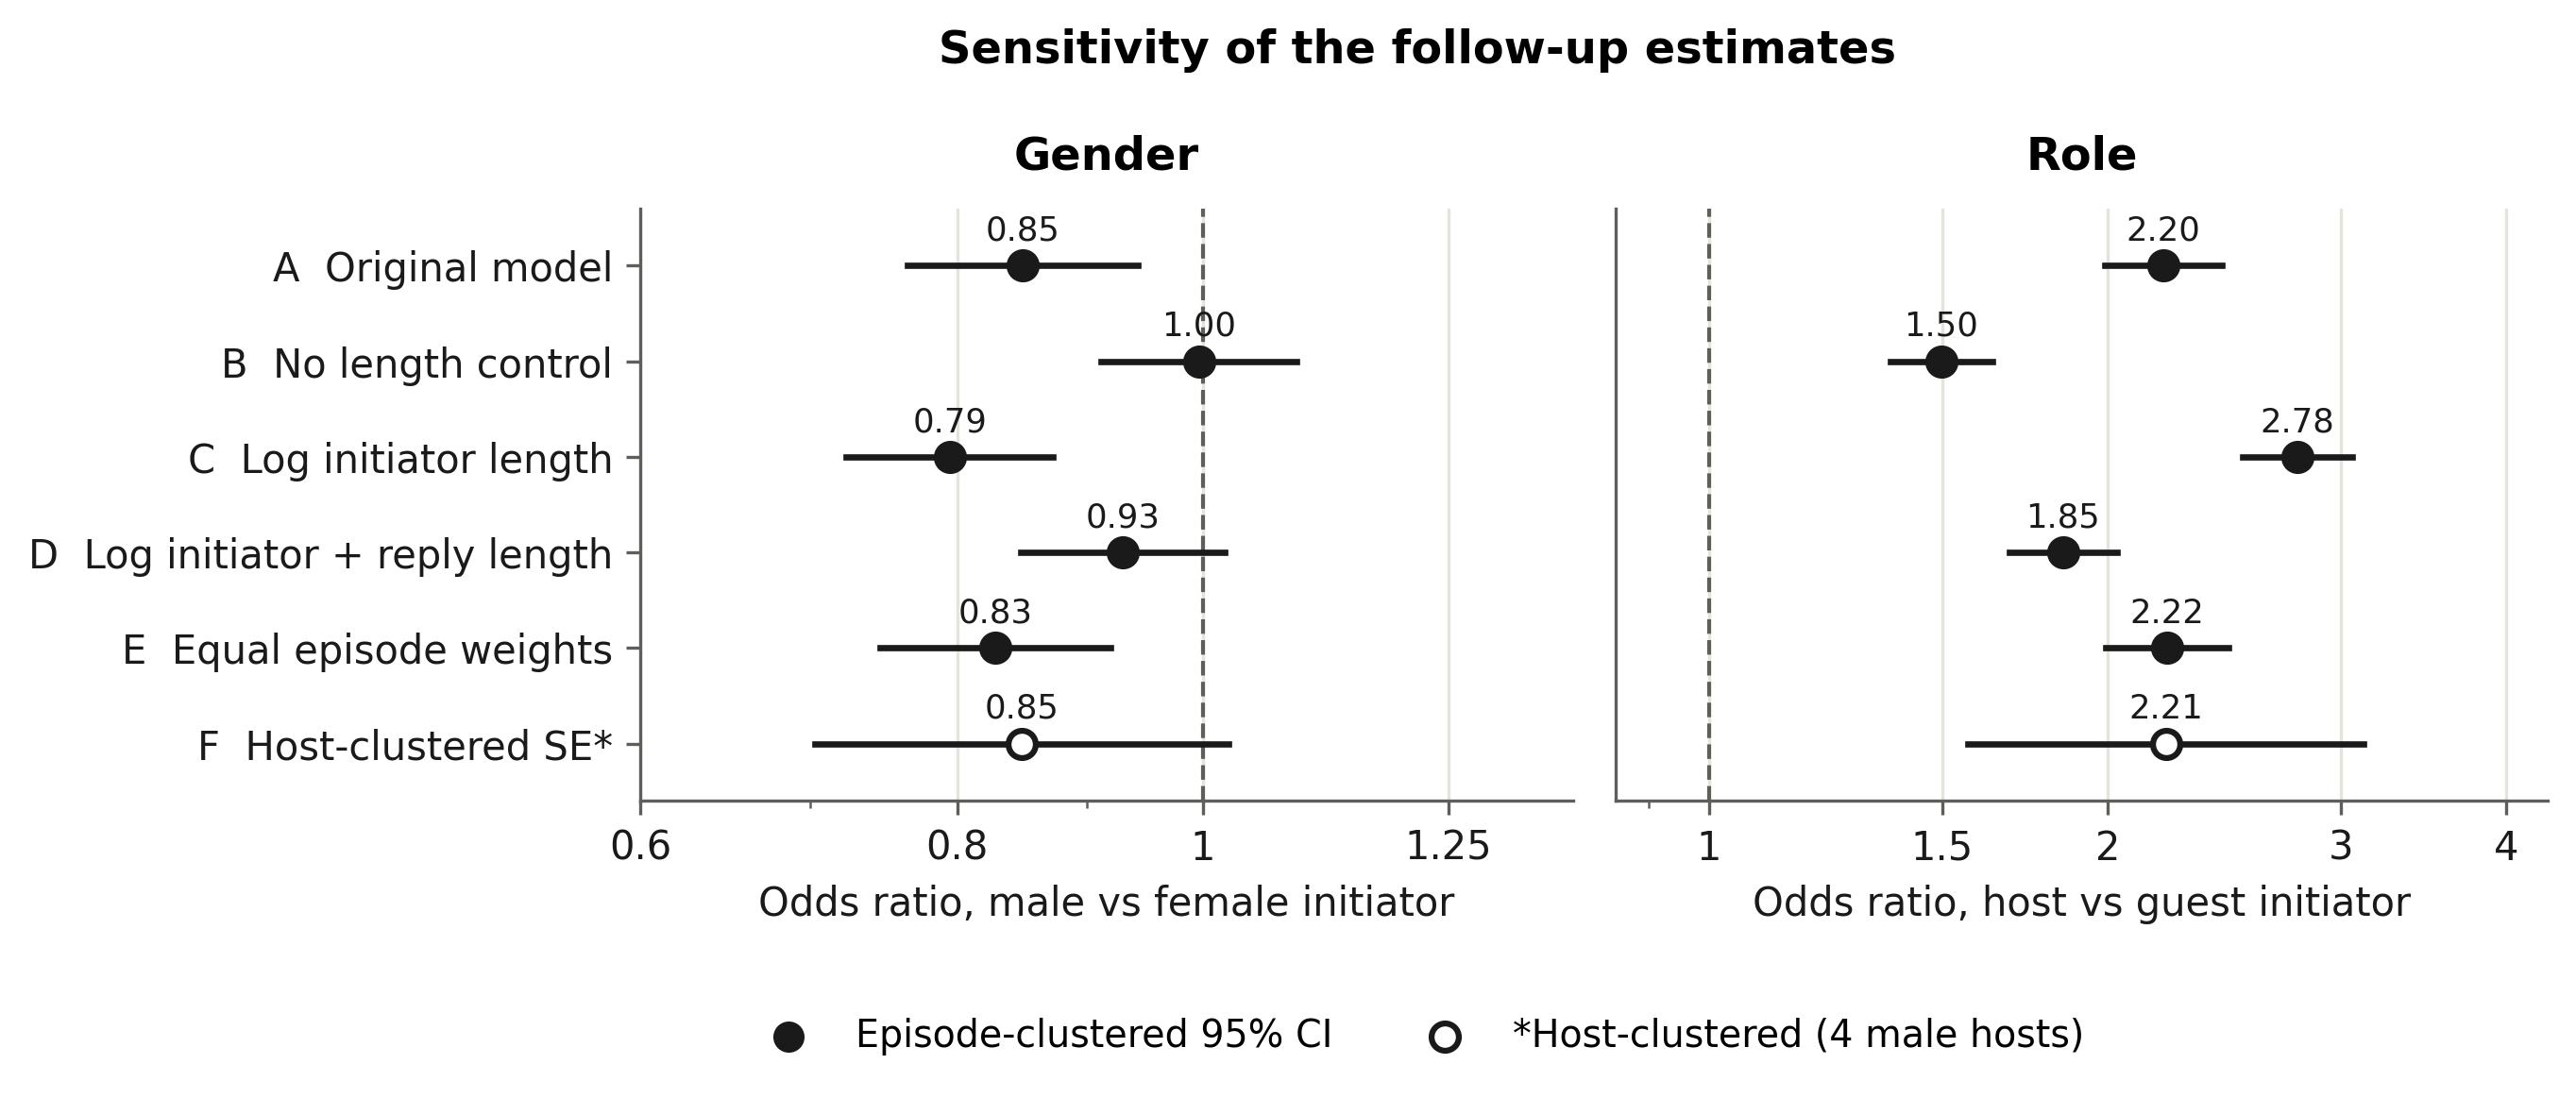
\includegraphics[width=0.9\linewidth]{figures/fig5_gender_estimate_sensitivity.png}
\caption{Gender (left) and role (right) odds ratios with 95\% CIs for binary lexical follow-up under the sensitivity models A--F of Table~\ref{tab:tc-sensitivity} (131 episodes). Filled markers: errors grouped by episode; open marker (F): errors grouped by host, shown for reference only. Log scale.}
\label{fig:tc-sensitivity}
\end{figure}

\paragraph{Role across all dyads:}
Across all episodes (42,320 initiations), host-initiated topics are followed up more than guest-initiated topics in every dyad (46--52\% vs.\ 36--41\%; Fig.~\ref{fig:tc-dyad}), whether the host is male or female. Part of this association comes from how the measure works: questions get more lexical follow-up than other turns, hosts ask more questions, and longer replies are more likely to share a word with the turn before them (Appendix Fig.~\ref{fig:tc-length}). So when a guest gives a long answer to a host's question, it usually counts as a follow-up.

\begin{figure}[H]
\centering
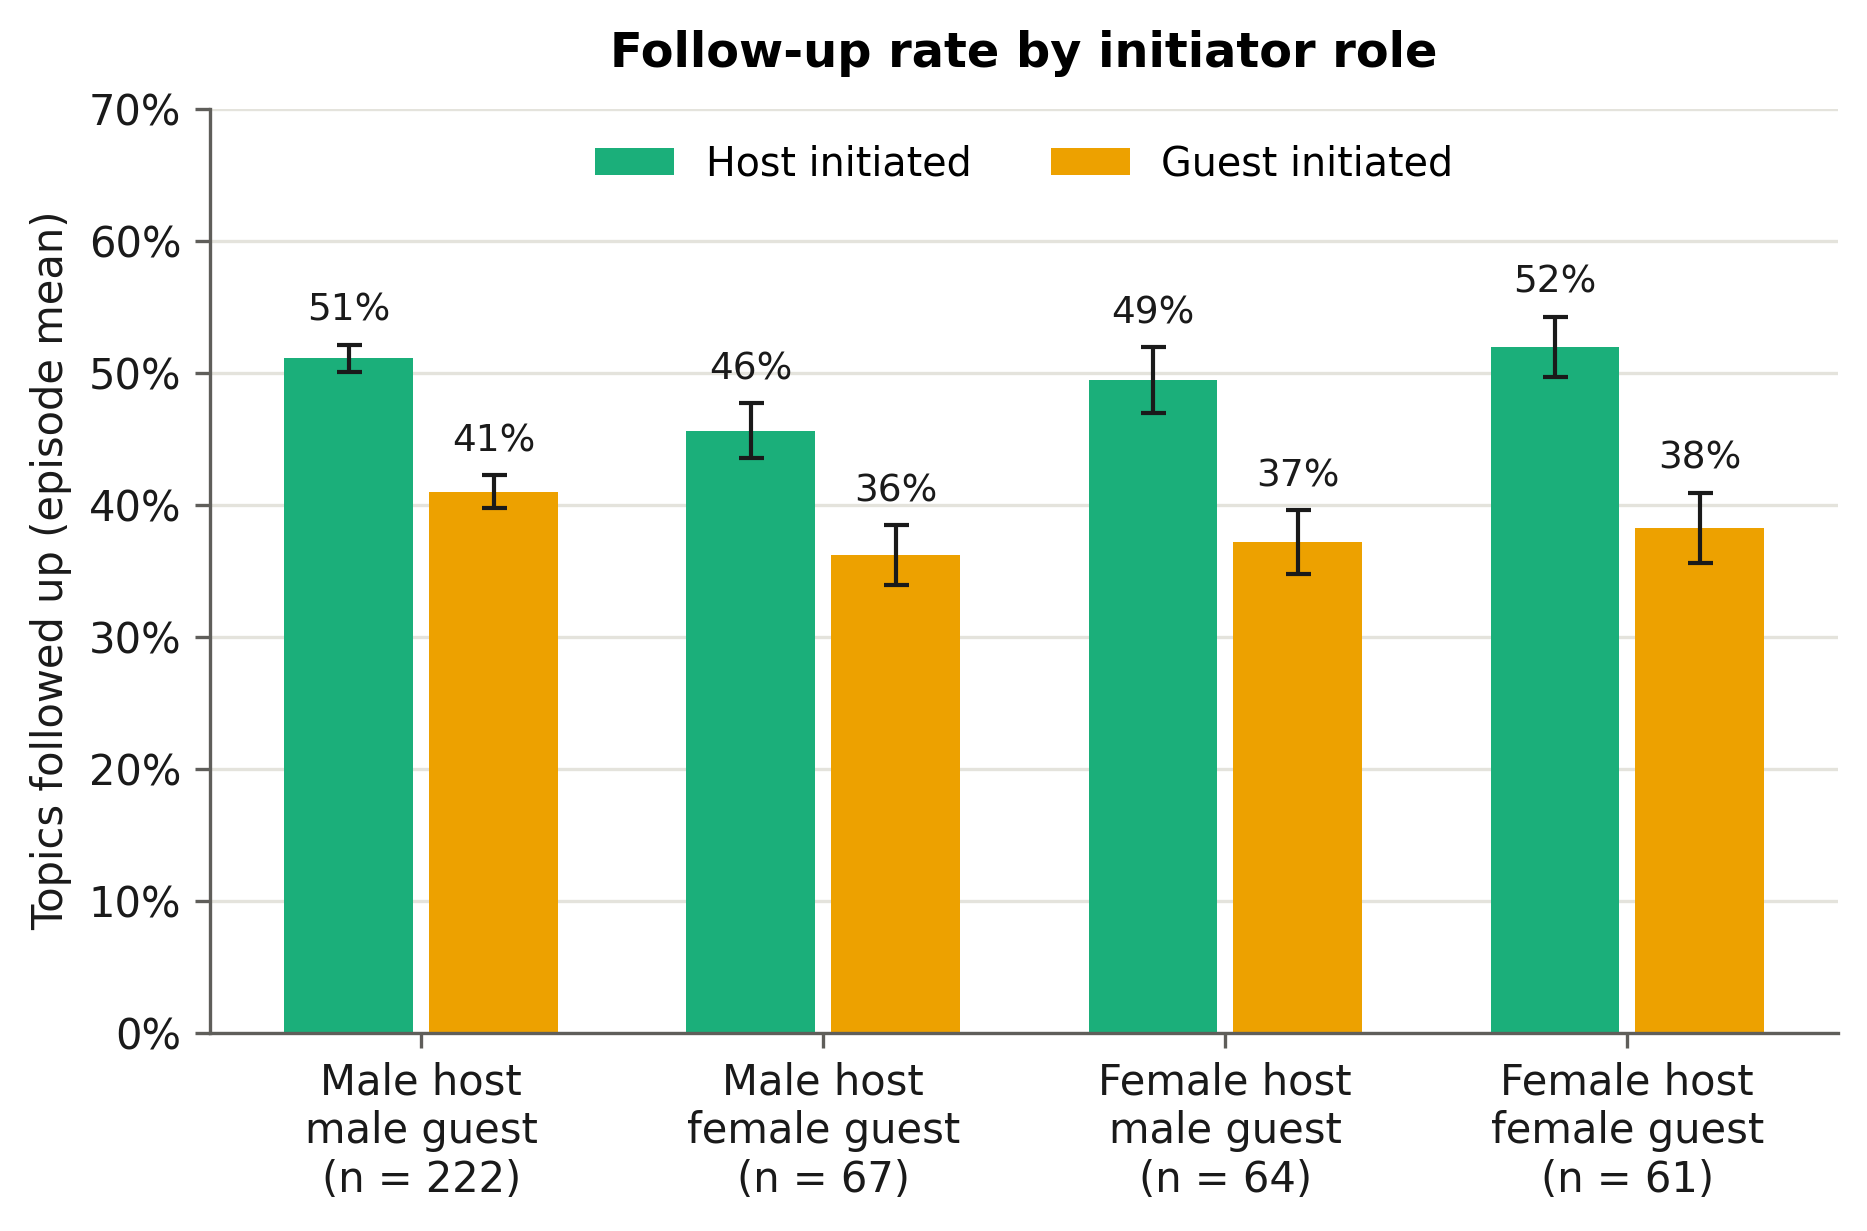
\includegraphics[width=0.75\linewidth]{figures/fig1_followup_by_role_all_dyads.png}
\caption{Automated lexical follow-up rate of host- and guest-initiated topics in each host$\rightarrow$guest dyad (414 episodes, 42,320 initiations; $n$ = episodes). Bars are means of episode-level rates with $t$-based 95\% CIs. Descriptive and unadjusted.}
\label{fig:tc-dyad}
\end{figure}

\subsubsection*{Limitations}
The measure is based on word overlap between neighbouring turns and has not been checked by human annotators, so it measures lexical uptake rather than topic follow-up as a listener would see it. Within an episode, gender and role cannot be separated. The mixed-gender episodes also come from only 4 male hosts and 4 named female hosts (plus 11 episodes whose host could not be identified), so the results may reflect particular shows more than gender. Reply length and question--answer structure also affect the measure.

\subsubsection*{Conclusion}
Our analysis found no evidence that men's topics are followed up more than women's. The male advantage in the pooled numbers mostly reflects role composition: men are usually the host in mixed-gender episodes, and hosts' topics receive more lexical follow-up. This host association is consistent across all dyads and models, but it is an association, not proof that role causes follow-up, and part of it comes from the question--answer format of interviews. Not finding support for H$_1$ also does not prove that gender has no effect: the gender result changes with how the model is set up, and it rests on a small number of hosts. The finding supports the idea that gendered speech patterns depend on context \cite{yoo2022conversational}. Without taking speaker role and episode grouping into consideration, the results could have wrongly suggested a gender bias.
